% ------------------------- MAIN TASK ---------------------------------
\section{Développement schématique}

\subsection{Choix des composants} \label{ssec:num32}
{
	\subsubsection{Microcontrôleur}
	Lors de la recherche de composants, j'ai décidé d'utiliser l'un des PIC32 standards de l'ES :
	\textbf{PIC32MX130F064D-I/PT}.
		
	\begin{figure}[h]
		\centering
		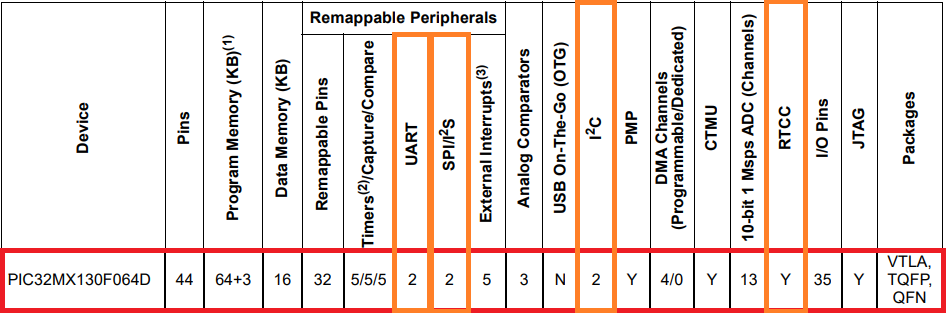
\includegraphics[width=1\linewidth]{Figures/Dev-SCH/PIC32-choisi}
		\caption{Périphériques disponibles du PIC}
		\label{fig:pic32-choisi}
		\source{PIC32MM0256GPM064 family datasheet}
	\end{figure}
	
	Nous pouvons constater sur la figure \ref{fig:pic32-choisi} que les critères minimaux de mon projet sont respectés :
	
	\begin{center}
		\fbox{\textit{1 - I2C}} \fbox{\textit{1 - SPI}} \fbox{\textit{1 - UART}} \fbox{\textit{1 - RTCC}}
	\end{center}
}

\clearpage
\subsection{Dimensionnements Hardware} \label{ssec:num31}
{
	\subsubsection{Vue d'ensemble schématique} \label{sssec:SchemaBloc} \vspace{-6mm}
	{
		\begin{figure}[th]
			\centering
			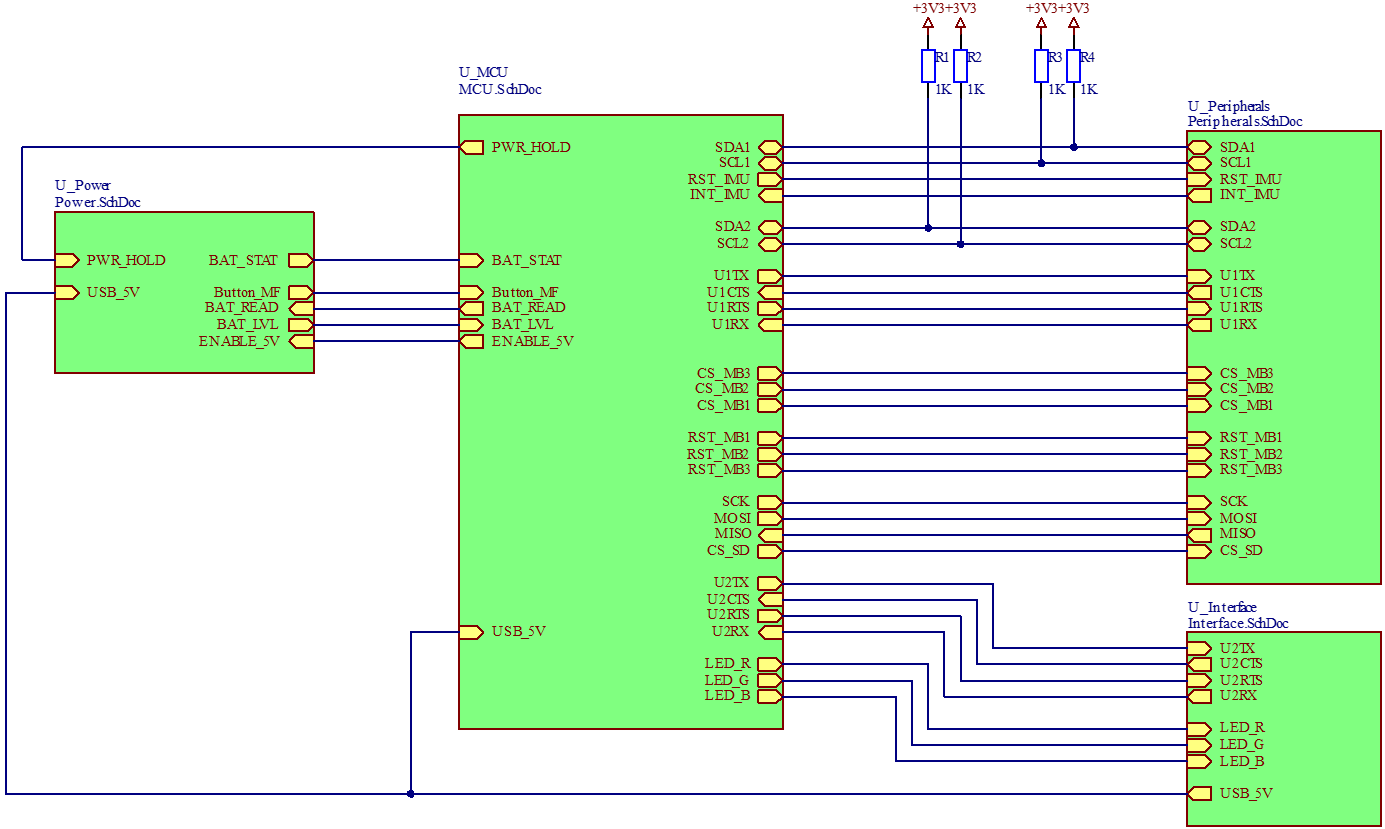
\includegraphics[width=1.1\linewidth]{Figures/Dev-SCH/schemaBloc}
			\caption{Schéma bloc de la schématique}
			\source{Auteur}
			\label{fig:schemablocSCH}
		\end{figure} \vspace{-5mm}
		Nous pouvons constater sur la figure \ref{fig:schemablocSCH} la structure des différents blocs du schéma : 
		
		\begin{tabularx}{18cm}{|X|X|}
			\hline
			Bloc & Description \\
			\hline
			\hline
			Power & Contient les différents régulateurs du système, ainsi que la gestion de charge de la batterie. \\
			\hline
			MCU & Contient l'intelligence du système, avec le microcontrôleur ainsi que tous ses composants passifs associés. \\
			\hline
			Peripherals & Périphériques du système : Carte-SD, Centrale inertielle, Capteur de pression, Slots MikroE. \\ 
			\hline
			Interface & Connecteur USB avec convertisseur serial (FTDI) et tous les composants passifs de sécurité. Interface LED RGB pour le statut. \\
			\hline
		\end{tabularx}
	}


	\clearpage
	\subsubsection{Autonomie du système} \label{sssec:SysAutonomie}
	{
		Afin de proportionner la batterie du circuit, il a fallut dimensionner les différentes consommations des composants, ceci par le biais de leurs documentations :
		
		\begin{center}
			\fbox{\textit{MCU - 30mA}} \fbox{\textit{BNO055 - 12.3mA}} \fbox{\textit{Capt. Pression - 4mA}} \fbox{\textit{\textcolor{red}{Carte-SD - 100mA}}} \fbox{\textit{MikroE - ??mA}} \fbox{\textit{Régulateurs - 40uA}} \fbox{\textit{LED RGB - 25mA}} 
		\end{center}
		
		Nous pouvons constater que la plus grande consommation vient de la carte micro-SD, qui au maximum peut induire 100mA. \footnote{Selon datasheet SanDisk : https://images-na.ssl-images-amazon.com/images/I/91tTtUMDM3L.pdf}
		
		
		Afin d'obtenir une autonomie d'au moins 2h (selon CDC), il faudrait une capacité de :
		
		\begin{equation}
			Capacite = Consommation_{tot} * Temps
		\end{equation}
		
		Ce qui nous fait une capacité de $\sim$342.68mAh, valeur facilement atteignable par les batteries li-ion du marché. Étant-donné que différents projets utilisaient des batteries 3400mAh, dans un objectif de conformité et de simplification des commandes, j'ai choisis cette même valeur.
		Ce qui signifie une autonomie de $\sim$20 heures, sans compter les différents mécanismes d'économie d'énergie.
		
		C'est un temps largement suffisant pour la durée de plusieurs expéditions, néanmoins la RTCC du microcontrôleur requiert d'être alimentée en permanence, j'ai donc décidé de déterminer un fonctionnement, où lorsque l'on charge la batterie la date se mettrait à jour et le mode "éteint" serait juste un mode de veille qui attendrait un niveau positif sur le switch avant de commencer le logging avec un timsetamp principale contenant la date, puis, seulement des deltas entre les mesures. Un diagramme des états est présents à la figure \ref{fig:etatsdiagramme}.
		
		\clearpage
		\begin{figure}[th]
			\centering
			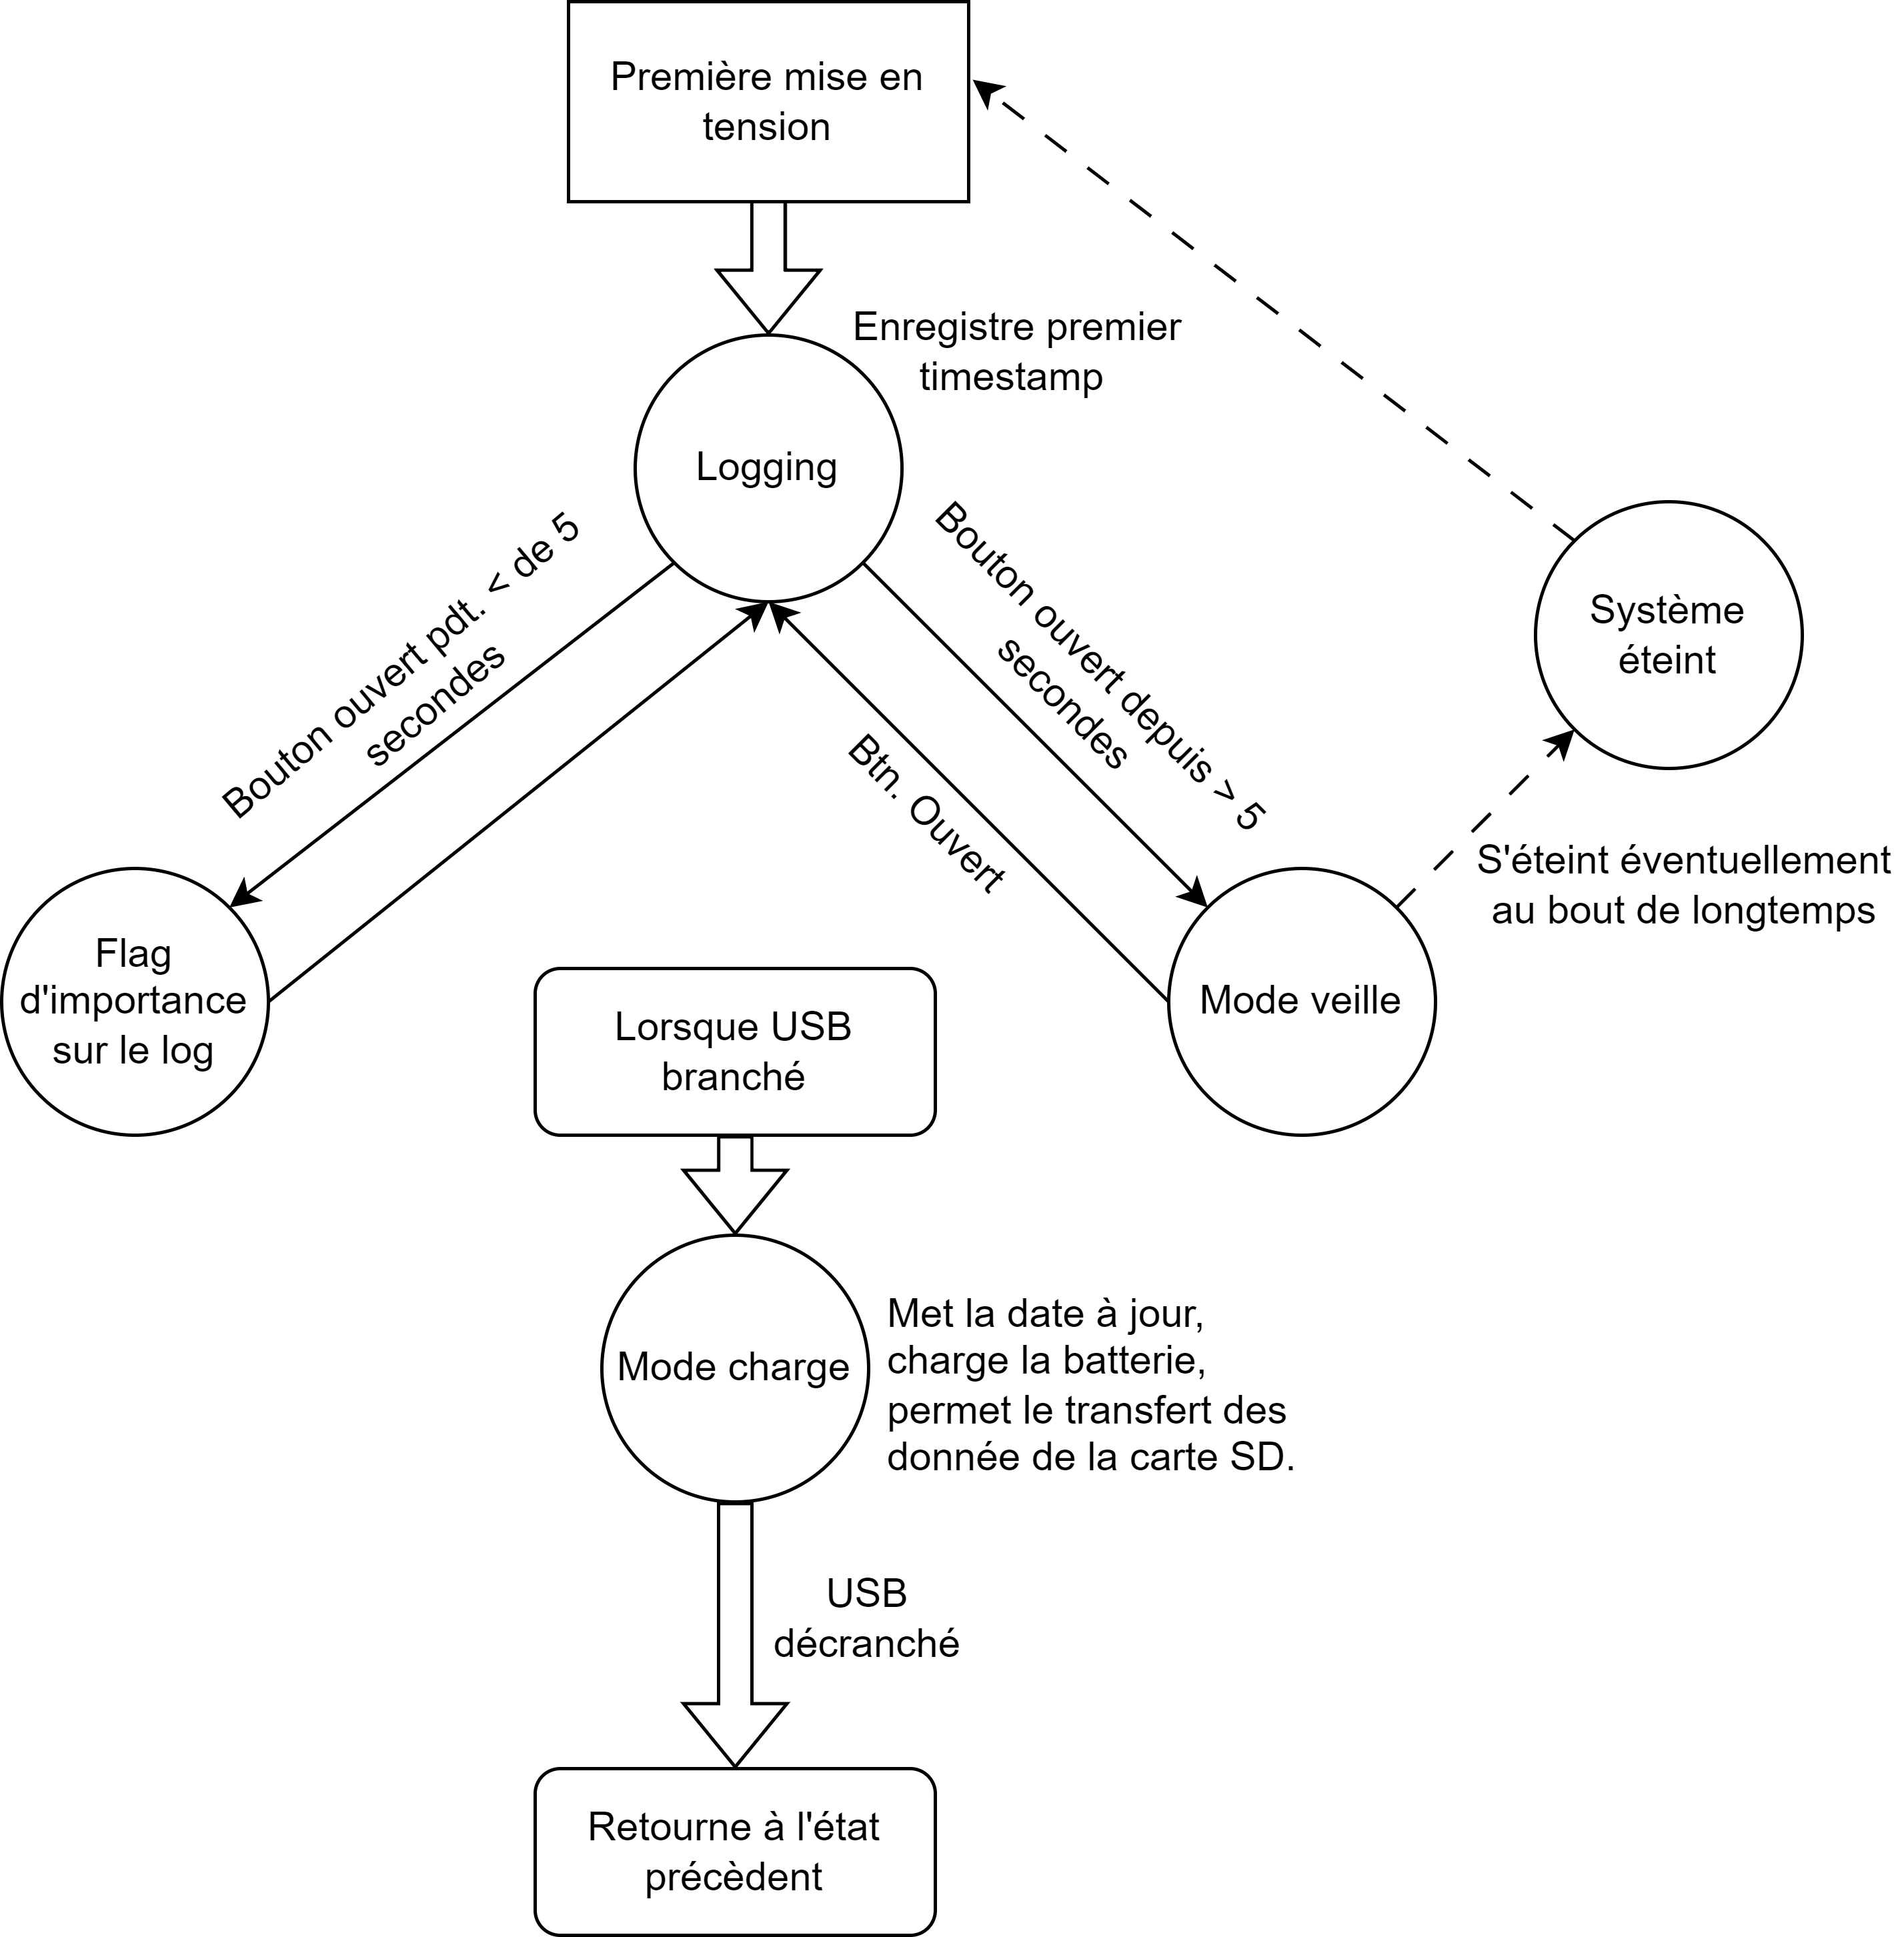
\includegraphics[width=1.1\linewidth]{Figures/Dev-SCH/Etats_diagramme}
			\caption{Diagramme des états du système}
			\label{fig:etatsdiagramme}
			\source{Auteur}
		\end{figure}
		
	}

	\clearpage
	\subsubsection{LED Interface} \label{sssec:DimLedRGB}
	{
		Afin d'informer l'utilisateur de ce qu'il se passe dans le système, j'ai décidé d'implémenter en tant qu'interface, une led RGB. Celle-ci sera un minimum puissante, afin de pouvoir être lisible lors de l'utilisation sous-marine du module.
		
		La consommation de la led RGB étant relativement importante, des mécanismes d'économie d'énergie seront mis en place dans le développement firmware. \vspace{+3mm}
		
		\textbf{Diagramme d'interface :}
		
		\begin{figure}[h]
			\centering
			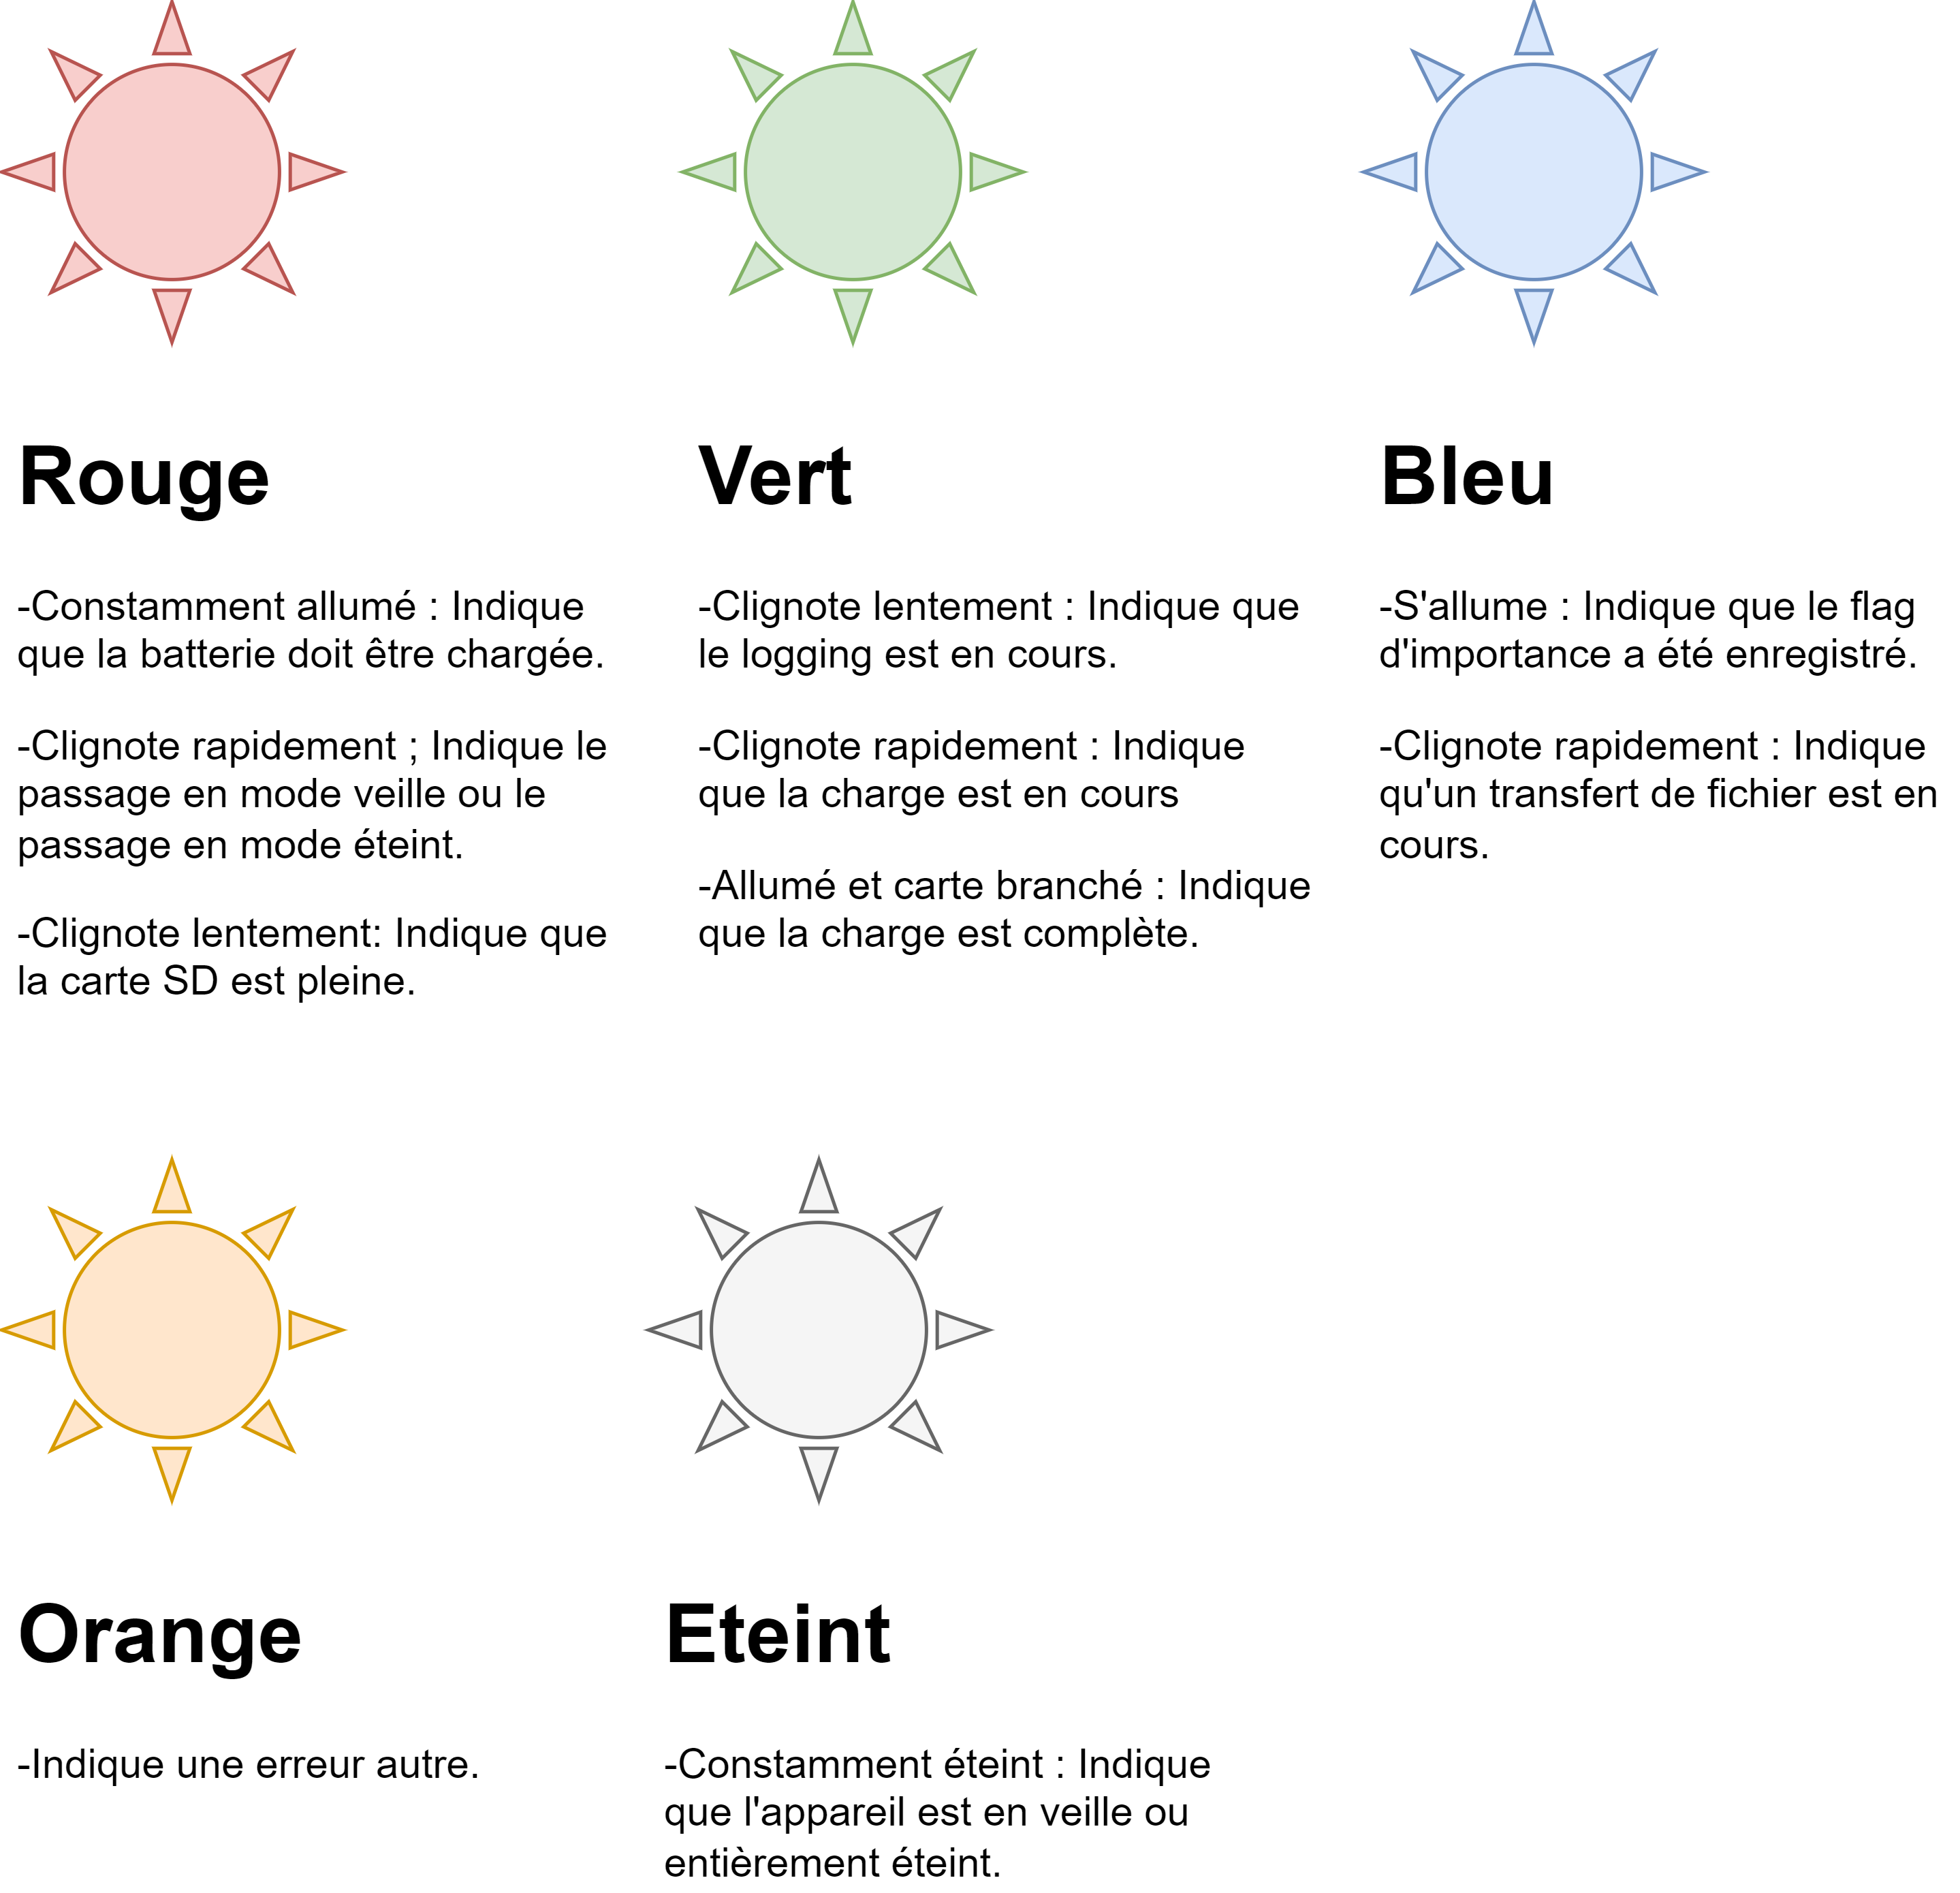
\includegraphics[width=0.95\linewidth]{Figures/Dev-SCH/LEDStates}
			\caption{Définitions des états de la LED RGB}
			\source{Auteur}
			\label{fig:ledstates}
		\end{figure}
	}

	\clearpage
	\subsubsection{Adaptation mécanique} \label{sssec:MecAdapt}
	{	
		L'idée étant d'obtenir une mesure de pression sans modification mécaniques sur le boîtier originale, plusieurs idées ont émergées : \\
		
		\begin{itemize}
			\item[1)] Mesurer une déformation mécanique a-même le module, dans le but de déduire la pression (Développement d'un capteur). \vspace{+2mm}
			
			\item[2)] Ajout d'une rallonge cylindrique au module, afin de fixer un capteur de pression à plat sur celui-ci, tout en permettant les modifications mécaniques sans altération du boîtier originale.
		\end{itemize}
		
		Par ordre de complexité et due aux contraintes de temps, la seconde option sera-celle développée.
	}

	\clearpage
	\subsubsection{Chargeur de batterie} \label{sssec:BatCharger}
	{
		
	}

	\subsubsection{Aspects techniques particuliers du schéma (bus, technologie particulière).}
	{
		
	}
	
	\subsubsection{Régulateur 3.3V} \label{sssec:Reg3V3}
	{
		
	}
	
	\subsubsection{Régulateur 5V} \label{sssec:Reg5V}
	{
		
	}
	

}


\clearpage